\documentclass[10pt, letterpaper]{paper}
\usepackage{graphicx}
\usepackage{amsmath}
\usepackage{amssymb}
\usepackage{mathrsfs}
\usepackage{float}

\title{ Operations Research Test 2 }
\author{ Timothy Schwieg }
\date{ November 29 2017 }

\begin{document}

\maketitle

\section*{Question 1 }
\begin{align*}
&-x_1 + 2x_2 -x_3 - 2x_4 \leq 0\\
&2x_1 - 3x_2 -x_3 + 3x_4 \leq 0\\
&-3x_1 +4x_2 + 3x_3 - 4x_4 < 0\\
\end{align*}
We may first note that the third inequality is strict, so we may add a new variable: $\epsilon > 0$ to the third constraint to make it non-strict.
\begin{align*}
&-x_1 + 2x_2 -x_3 - 2x_4 \leq 0\\
&2x_1 - 3x_2 -x_3 + 3x_4 \leq 0\\
&-3x_1 +4x_2 + 3x_3 - 4x_4 + \epsilon \leq 0\\
&\epsilon > 0\\
\end{align*}
This can be written as:

\[ \left ( { \begin{array}{ccccc}
	-1 & 2 & -1 & -2 & 463487 \\
	2 & -3 & -1& 3 & 0\\
	-3 & 4 & 3 & -3 & 1\\
	\end{array}}\right) 
	\left( { \begin{array}{c}
	x\\
	\epsilon\\
	\end{array}} \right )
	\leq \left( { \begin{array}{c}
	0\\
	0\\
	0\\
	\end{array}} \right ) \text{ and: } \left( { \begin{array}{c}
	0\\
	0\\
	0\\
	0\\
	1\\
	\end{array}} \right)^T 
	\left( { \begin{array}{c}
	x\\
	\epsilon\\
	\end{array}} \right ) > \left( { \begin{array}{c}
	0\\
	0\\
	0\\
	0\\
	0\\
	\end{array}}\right ) \]
	
	
By Farkas' Lemma, this does not have a solution if $A^T y = c$ has a solution for $y \geq 0$.

\[
\left ( { \begin{array}{ccccc}
	-1 & 2 & -1 & -2 & 0 \\
	2 & -3 & -1& 3 & 0\\
	-3 & 4 & 3 & -3 & 1\\
	\end{array}}\right)^T y =  \left( { \begin{array}{c}
	0\\
	0\\
	0\\
	0\\
	1\\
	\end{array}} \right)
\]

We can solve this system and we arrive at:
\[
y = \left ( {\begin{array}{c}
	1\\
	2\\
	1\\
	\end{array}} \right ) \geq 0 \]
	
Since we found a weakly positive solution for y, Farkas' Lemma informs us that there is no solution to the inequality system.

\section*{Question 2}
\begin{equation*}
\begin{alignedat}{3}
&\text{max }&5x_1 + 4x_2&\\
&\text{s.t. } &6x_1 + 4x_2 &\leq 24\\
& &x_1 + 2x_2 &\leq 6\\
& &0x_1 + x_2 &\leq 2\\
& &-x_1 + x_2 &\leq 1\\
& &x_1, x_2 &\geq 0
\end{alignedat}
\end{equation*}
Putting in Tableau form:

\[
	\left[ {\begin{array}{ccccccc|c}
	Z & x_1 & x_2 & s_1 & s_2 & s_3 &s_4 & RHS\\ \cline{1-8}
	1 & -5 & -4 & 0 & 0 & 0 & 0 & 0 \\
	0 & 6 & 4 & 1 & 0 &0 & 0 &24\\
	0 & 1 & 1 & 0& 1 & 0 &0 & 6\\
	0 & 0 & 1 & 0 & 0 & 1 &0 & 2 \\
	0 & -1 & 1 & 0 & 0 & 0 &1 & 1 \\
	\end{array} } \right]
\]
This becomes:
\[
	\left[ {\begin{array}{ccccccc|c}
	Z & x_1 & x_2 & s_1 & s_2 & s_3 &s_4 & RHS\\ \cline{1-8}
	1 & 0 & 0 & \frac{3}{4} & \frac{1}{2} & 0 & 0 & 21\\
	0 & 1 & 0 & \frac{1}{4} & \frac{-1}{2} &0 & 0 &3\\
	0 & 0 & 1 & \frac{-1}{8}& \frac{3}{4} & 0 &0 & \frac{3}{2}\\
	0 & 0 & 0 & \frac{1}{8} & \frac{-3}{4} & 1 &0 & \frac{1}{2} \\
	0 & 0 & 0 & \frac{3}{8} & \frac{-5}{4} & 0 &1 & \frac{5}{2} \\
	\end{array} } \right]
\]

Taking a Gomory Cut based on the basic variable $s_3$.

\begin{align*}
\frac{1}{8} s_1 - \frac{3}{4} s_2 + s_3 &= \frac{1}{2}\\
(0 + \frac{1}{8}) s_1 + ( -1 + \frac{1}{4} )s_2 + (1 + \frac{0}{1})s_3 &= ( 0 + \frac{1}{2} )\\
\frac{1}{8} s_1 +\frac{1}{4} s_2 \geq \frac{1}{2}\\
s_1 + 2s_2 \geq 4\\
\end{align*}
Applying this cut we get: 
\begin{equation*}
\begin{alignedat}{3}
&\text{max }&5x_1 + 4x_2&\\
&\text{s.t. } &6x_1 +4x_2 + s_1 &= 24\\
& &x_1 + 2x_2 + s_2 &= 6\\
& &0x_1 + x_2 &\leq 2\\
& &-x_1 + x_2 &\leq 1\\
& & s_1 + 2s_2 &\geq 4\\
& &x_1, x_2 &\geq 0
\end{alignedat}
\end{equation*}

This yeilds the solution:Z = 20 located at $x_1 = 4, x_2 = 0, s_1 = 0, s_2 = 2$ Note that this is an integer solution and the problem states that two iterations are to be done only ``IF NEEDED," as they are not needed they will not be done.

\section*{Question 3.}
\begin{equation*}
\begin{alignedat}{4}
&\text{min }&x_1^2 +x_2^2 + x_3^2&\\
&\text{s.t. } &2x_1 +x_2 &\leq 5 \quad &(1)\\
& &x_1 + x_3 &\leq 2 \quad &(2)\\
& &x_1 &\geq 1 \quad &(3)\\
& &x_2 &\geq 2 \quad &(4)\\
& &x_3 &\geq 0 \quad &(5)\\
\end{alignedat}
\end{equation*}
Our point to verify is: $x = (1,2,0)$
First we can check primal feasibility:
\begin{align*}
(1) \quad& 2(1)+2 = 4 \leq 4\\
(2) \quad& 1 + 0 = 1 \leq 2\\
(3) \quad& 1 \geq 1\\
(4) \quad& 2 \geq 2\\
(5) \quad& 0 \geq 0\\
\end{align*}
Now we can consider dual feasibility: Note that only constraints (3),(4),(5) bind.
\newline
Checking dual feasibility:
\[ \nabla f = \left ( {\begin{array}{c}
	2x_1\\
	2x_2\\
	2x_3\\
	\end{array} } \right ) \quad \nabla g_3 = \left ( {\begin{array}{c}
	-1\\
	0\\
	0\\
	\end{array} } \right ) \quad \nabla g_4 = \left ( {\begin{array}{c}
	0\\
	-1\\
	0\\
	\end{array} } \right ) \quad \nabla g_5 = \left ( {\begin{array}{c}
	0\\
	0\\
	-1\\
	\end{array} } \right ) \]
	It is obvious that the constraints g are linearly independent, as they are orthogonal.
\[ 
\left ( {\begin{array}{c}
	2\\
	4\\
	0\\
	\end{array} } \right ) + \left ( {\begin{array}{c}
	-u_3\\
	0\\
	0\\
	\end{array} } \right ) + \left ( {\begin{array}{c}
	0\\
	-u_4\\
	0\\
	\end{array} } \right ) + \left ( {\begin{array}{c}
	0\\
	0\\
	-u_5\\
	\end{array} } \right ) = 0
\]
These solutions imply that: $u_3 = 2, u_4 = 4, u_5 = 0$. It is clear that the first two constraints do not bind, so $u_1 = u_2 = 0$
Immedietly complementary slackness is satisfied in the first two constraints and the fifth, so we need only verify (3) and (4)
\begin{align*}
(1) \quad& 2( 1 - x_1 ) = 2( 1 - 1 ) = 0\\
(2) \quad& 4(2-x_2 ) = 4( 2-2) = 0\\
\end{align*}
Since all the u's are all weakly positive, it is a KKT point.

\section*{Question 4}
Let $X_i$ indicate the number of officers that begin their double shift at time index i.
\begin{equation*}
\begin{alignedat}{3}
&\text{min }&x_0 + x_1 + x_2 + x_3 + x_4 + x_5&\\
&\text{s.t. } &x_5 + x_0 &\geq 8\\
& &x_0 + x_1 &\geq 7\\
& &x_1 + x_2 &\geq 6\\
& &x_2 + x_3 &\geq 6\\
& &x_3 + x_4 &\geq 5\\
& &x_4 + x_5 &\geq 4\\
& &x_i \in \mathbb{Z}_+ &\\
\end{alignedat}
\end{equation*}
\subsection*{b}
Solving the relaxed Linear Program:
\begin{equation*}
\begin{alignedat}{3}
&\text{min }&x_0 + x_1 + x_2 + x_3 + x_4 + x_5&\\
&\text{s.t. } &x_5 + x_0 &\geq 8\\
& &x_0 + x_1 &\geq 7\\
& &x_1 + x_2 &\geq 6\\
& &x_2 + x_3 &\geq 6\\
& &x_3 + x_4 &\geq 5\\
& &x_4 + x_5 &\geq 4\\
& &x_i \in \mathbb{R}_+ &\\
\end{alignedat}
\end{equation*}
This yeilds solution Z = 19 located at x=(2,5,1,5,0,6). Since this has all integer values, it is optimal for the integer program. Again, since branch and bound steps are not necessary, and the problem states ``if needed" we will not do any steps.

\section*{Question 5.}
Firstly we may note that this is an M/M/1/25 Queue with parameters: $\lambda = \frac{1}{2}, \mu = \frac{ 1}{3}, \rho = \frac{3}{2}$
\begin{equation*}
\begin{alignedat}{2}
p_0 &= \frac{ 1 - \rho }{ 1- \rho^{26} } = \frac{ 2^{25}}{ 3^{26} - 2^{26} } &\approx 0.00001320\\
p_{25} &= \rho^{25} p_0 = \frac{ 3^{25} } { 3^{26} - 2^{26} } &\approx 0.333342\\
\lambda_{eff} &= \lambda ( 1- p_{25} ) \approx \frac{1}{2} ( 1 - .333342 ) &\approx 0.3333289\\
L_s &= \frac{ \rho[ 1 - 26 \rho^{25} + 25 \rho^{26} ] }{ (1-\rho)(1-\rho^{26})} &\approx 23.000686\\
W_s &= \frac{ L_s } { \lambda_{eff}} &\approx 69.002977\\
W_q &= W_s - \frac{1}{\mu} &\approx 66.00297710\\
L_q &= \lambda_{eff} W_q &\approx 22.0007\\
\end{alignedat}
\end{equation*}
\subsection*{a}
$$p_0 \approx 0.00001320$$
\subsection*{b}
$$L_q \approx 22.0007$$
\subsection*{c}
$$W_s \approx 69.002977$$
\subsection*{d}
Now the problem has become an M/M/2/25 Queue.
$$\lambda = \frac{1}{2}, \mu = \frac{1}{3}, \rho = \frac{3}{2}, N = 25, c = 2$$
\begin{equation*}
\begin{alignedat}{2}
p_0 &= ( 1 + \rho + \frac{ \rho^s ( 1 - \frac{\rho}{c}^{N-c+1} ) }{ c! ( 1 - \frac{ \rho }{c})})^{-1} &\approx .14295\\
p_{25} &= p_0 \frac{ \rho^{25} }{ c! c^{N-c} } = \frac{3^{25}}{2^{49}} p_0 &\approx .00021515\\
L_q &= \frac{ \rho^{c+1} }{ (c-1)!(c-\rho)^2}[ 1 - \frac{ \rho}{c}^{N-c+1} - (N-c+1)(1-\frac{\rho}{c})(\frac{ \rho}{c})^{N-c} ]p_0 &\approx 1.9124\\
\lambda_{eff} &= (1-p_{25})\lambda &\approx .49989\\
W_q &= \frac{ L_q}{\lambda_{eff}} &\approx 3.8256\\
W_s &= W_q + \frac{ 1}{\mu} &\approx 6.8256\\
\end{alignedat}
\end{equation*}

\section*{Question 6.}
\begin{figure}[H]
\centering
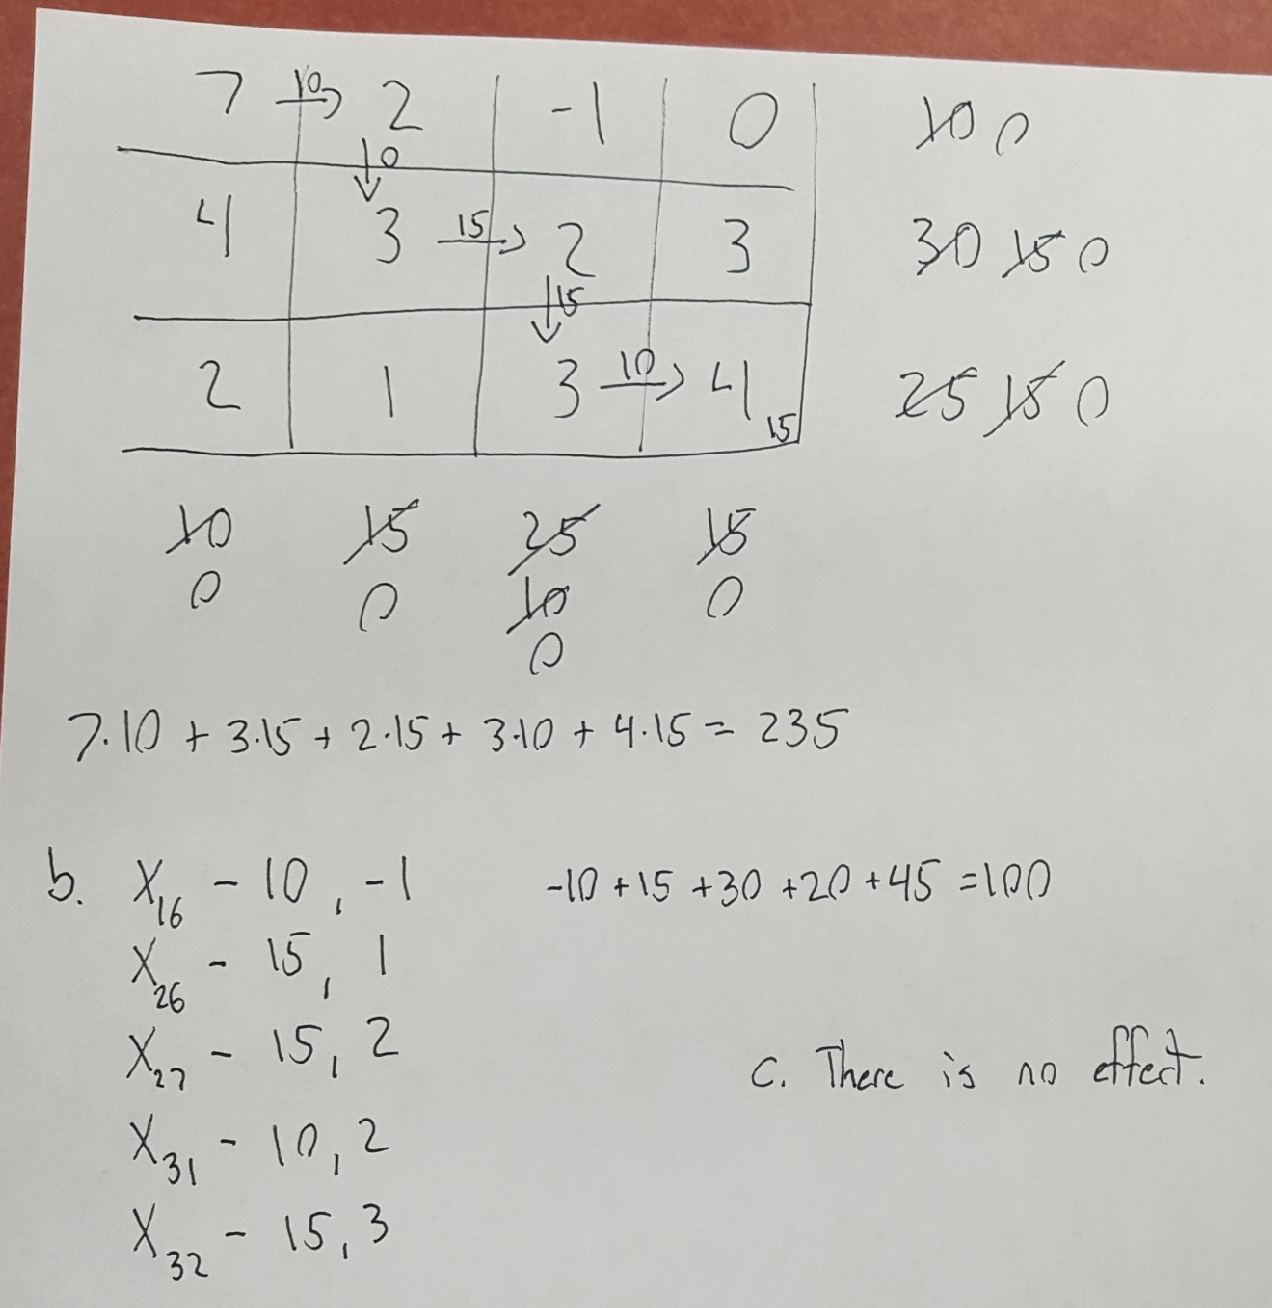
\includegraphics[width=1.0\textwidth]{Resized_20171130_191552.jpeg}
\caption{ Question 6 }
\end{figure}
\end{document}
